\documentclass[11pt,a4paper]{article}

% Packages
\usepackage[utf8]{inputenc}
\usepackage[T1]{fontenc}
\usepackage{amsmath,amssymb,amsfonts}
\usepackage{graphicx}
\usepackage{geometry}
\usepackage{hyperref}
\usepackage{listings}
\usepackage{xcolor}
\usepackage{float}
\usepackage{booktabs}
\usepackage{caption}
\usepackage{subcaption}
\usepackage{enumitem}

\geometry{margin=1in}

% Code listing style
\lstset{
    language=Python,
    basicstyle=\ttfamily\small,
    keywordstyle=\color{blue}\bfseries,
    stringstyle=\color{red},
    commentstyle=\color{gray}\itshape,
    numbers=left,
    numberstyle=\tiny\color{gray},
    stepnumber=1,
    numbersep=5pt,
    backgroundcolor=\color{gray!5},
    frame=single,
    rulecolor=\color{gray!30},
    breaklines=true,
    breakatwhitespace=false,
    tabsize=4,
    showstringspaces=false,
    captionpos=b
}

\title{\textbf{CSE 8803: CMC --- Assignment 2}}
\author{}
\date{}

\begin{document}
\maketitle

%% ====================================================================
%% QUESTION 1
%% ====================================================================
\section{Gephi Visualization}

The network dataset chosen for this visualization is the \textbf{US Airport} network, which represents flight routes between airports in the United States. Nodes correspond to airports and edges correspond to direct flight connections between them.

The visualization was created using Gephi with the following settings:
\begin{itemize}
    \item \textbf{Layout:} ForceAtlas 2 (for spatial separation of clusters)
    \item \textbf{Node size:} Scaled by degree centrality (hub airports appear larger)
    \item \textbf{Edge color:} Gradient based on edge weight
\end{itemize}

The resulting visualization clearly shows the hub-and-spoke structure characteristic of the US airline network, with major hubs (e.g., ATL, ORD, DFW) having significantly higher connectivity.

\begin{figure}[H]
    \centering
    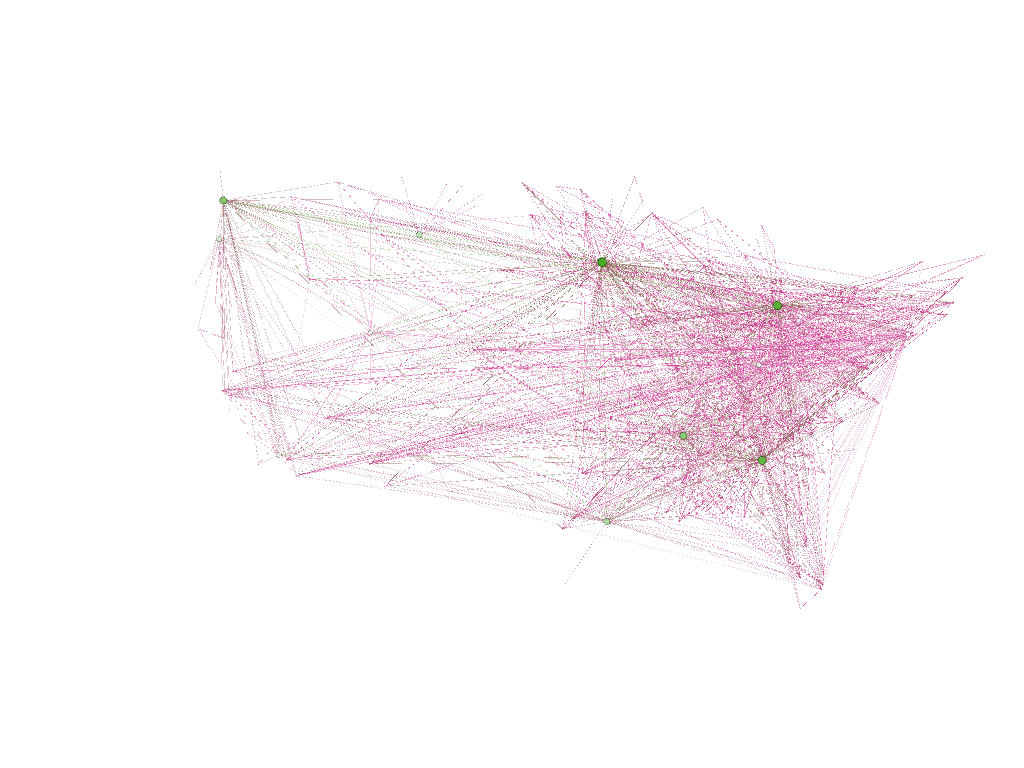
\includegraphics[width=0.85\textwidth]{output/q1_visualization_US_airports.png}
    \caption{Gephi visualization of the US Airport network. Node size reflects degree centrality; edge colors represent route density.}
    \label{fig:q1_gephi}
\end{figure}

%% ====================================================================
%% QUESTION 2
%% ====================================================================
\section{Small World Networks}

%% ---- 2(a) ----
\subsection{(a) Constructing a Small World Network}

\subsubsection*{Network Class Implementation}

The \texttt{UndirectedGraph} class stores the graph as a dictionary mapping each node to its list of neighbors. The five required functions are implemented as follows:

\begin{lstlisting}[caption={HasNode and AddNode}]
def HasNode(self, node):
    return node in self.connections

def AddNode(self, node):
    if not self.HasNode(node):
        self.connections[node] = []
\end{lstlisting}

\begin{lstlisting}[caption={AddEdge --- adds nodes first, then creates undirected edge if it does not exist}]
def AddEdge(self, node1, node2):
    self.AddNode(node1)
    self.AddNode(node2)
    if node2 not in self.connections[node1]:
        self.connections[node1].append(node2)
        self.connections[node2].append(node1)
\end{lstlisting}

\begin{lstlisting}[caption={GetNodes and GetNeighbors}]
def GetNodes(self):
    return list(self.connections.keys())

def GetNeighbors(self, node):
    return self.connections[node][:]   # return a copy
\end{lstlisting}

\subsubsection*{Small World Network Construction}

The ring graph is built by connecting each node $i$ to nodes $(i+j) \bmod L$ for $j = 1, \ldots, Z/2$. Because the graph is undirected, each \texttt{AddEdge} call automatically creates both directions, so iterating only over positive offsets suffices. The modulo operation implements periodic boundary conditions.

\begin{lstlisting}[caption={MakeRingGraph}]
def MakeRingGraph(num_nodes, Z):
    g = networks.UndirectedGraph()
    for i in range(num_nodes):
        g.AddNode(i)
    for i in range(num_nodes):
        for j in range(1, Z // 2 + 1):
            neighbor = (i + j) % num_nodes
            g.AddEdge(i, neighbor)
    return g
\end{lstlisting}

Random shortcuts are added by selecting two distinct nodes uniformly at random. The \texttt{AddEdge} function internally prevents duplicate edges.

\begin{lstlisting}[caption={MakeSmallWorldNetwork (Watts--Newman variant)}]
def MakeSmallWorldNetwork(L, Z, p):
    g = MakeRingGraph(L, Z)
    num_shortcuts = int(p * Z * L / 2)
    AddRandomEdges(g, num_shortcuts)
    return g
\end{lstlisting}

\subsubsection*{Verification of Periodic Boundary Conditions}

For $L=20$, $Z=4$, $p=0.2$:
\begin{itemize}
    \item Node 0 neighbors: $\{1, 2, 18, 19, \ldots\}$ (includes ring wrapping plus random shortcuts)
    \item Node 19 neighbors: $\{0, 1, 17, 18, \ldots\}$ (correctly wraps around)
\end{itemize}

Figure~\ref{fig:q2a} shows the network with gray ring edges and red shortcut edges.

\begin{figure}[H]
    \centering
    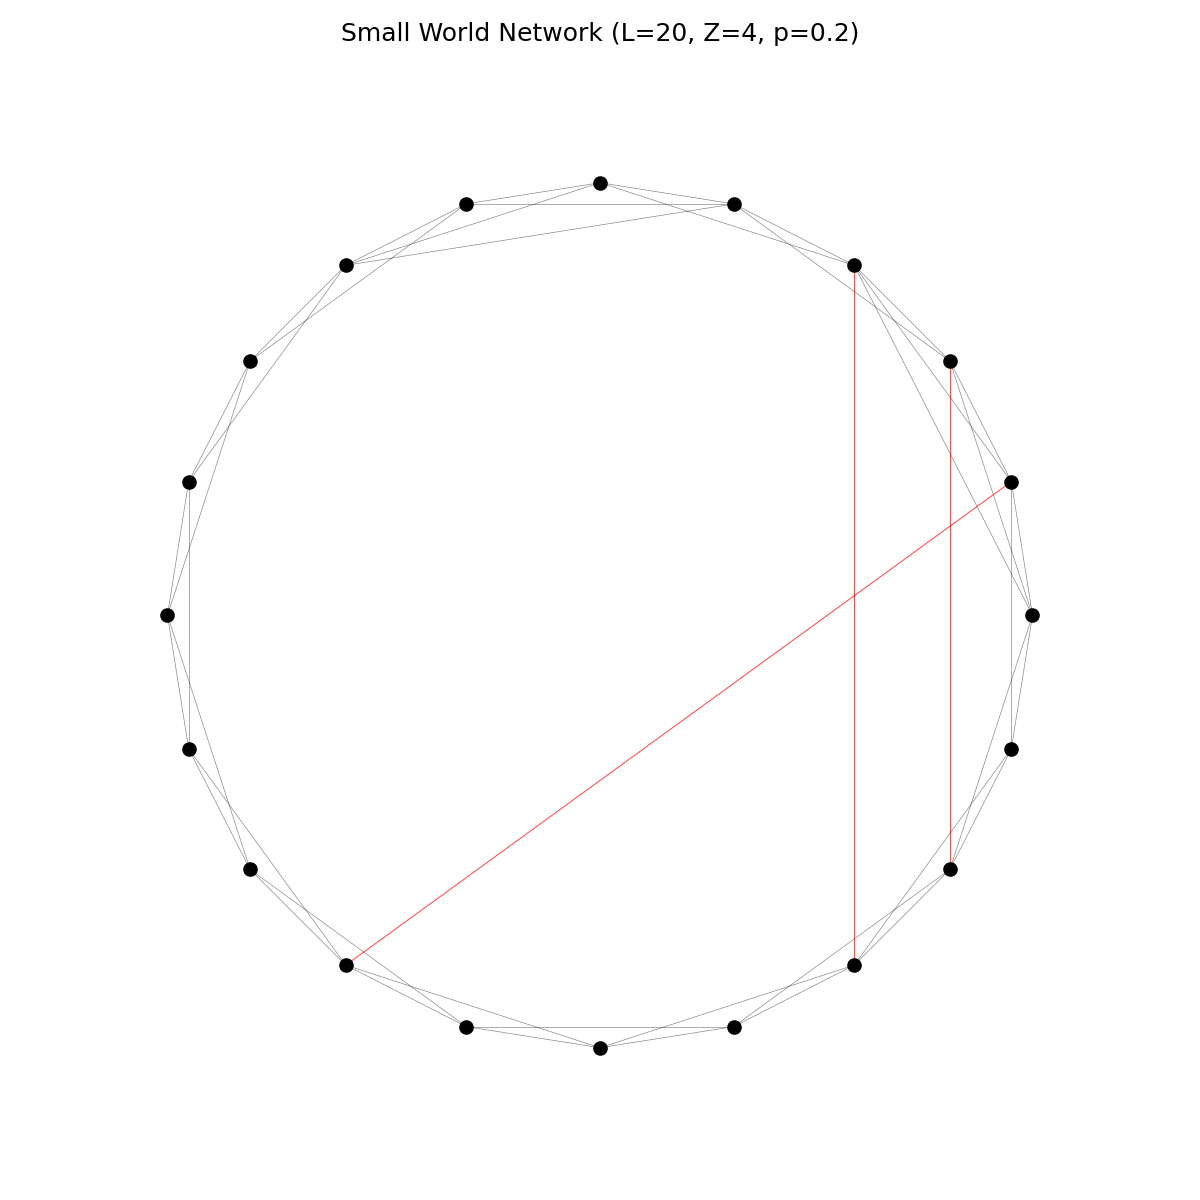
\includegraphics[width=0.55\textwidth]{output/q2a_smallworld_L20_Z4_p02.png}
    \caption{Small world network with $L=20$, $Z=4$, $p=0.2$. Gray edges are ring connections; red edges are random shortcuts.}
    \label{fig:q2a}
\end{figure}

%% ---- 2(b) ----
\subsection{(b) Measuring Minimum Distances Between Nodes}

\subsubsection*{BFS Algorithm}

\texttt{FindPathLengthsFromNode} implements a breadth-first search that expands outward in shells:

\begin{lstlisting}[caption={FindPathLengthsFromNode --- BFS}]
def FindPathLengthsFromNode(graph, node):
    distances = {node: 0}
    l = 0
    currentShell = [node]
    while currentShell:
        nextShell = []
        for currentNode in currentShell:
            for neighbor in graph.GetNeighbors(currentNode):
                if neighbor not in distances:
                    distances[neighbor] = l + 1
                    nextShell.append(neighbor)
        l += 1
        currentShell = nextShell
    return distances
\end{lstlisting}

\texttt{FindAllPathLengths} calls the BFS from every node and collects all pairwise distances. \texttt{FindAveragePathLength} averages over all pairs.

\begin{lstlisting}[caption={FindAllPathLengths and FindAveragePathLength}]
def FindAllPathLengths(graph):
    allLengths = {}
    for node in graph.GetNodes():
        distances = FindPathLengthsFromNode(graph, node)
        for node2, dist in distances.items():
            if node != node2:
                allLengths[(node, node2)] = dist
    return allLengths

def FindAveragePathLength(graph):
    allLengths = FindAllPathLengths(graph)
    if len(allLengths) == 0:
        return 0
    return sum(allLengths.values()) / len(allLengths)
\end{lstlisting}

\subsubsection*{Verification at $p=0$}

For a ring graph ($p=0$) with $L=100$, $Z=2$, path lengths range from $1$ to $L/Z = 50$, and the histogram is constant (uniform), as expected.

\begin{figure}[H]
    \centering
    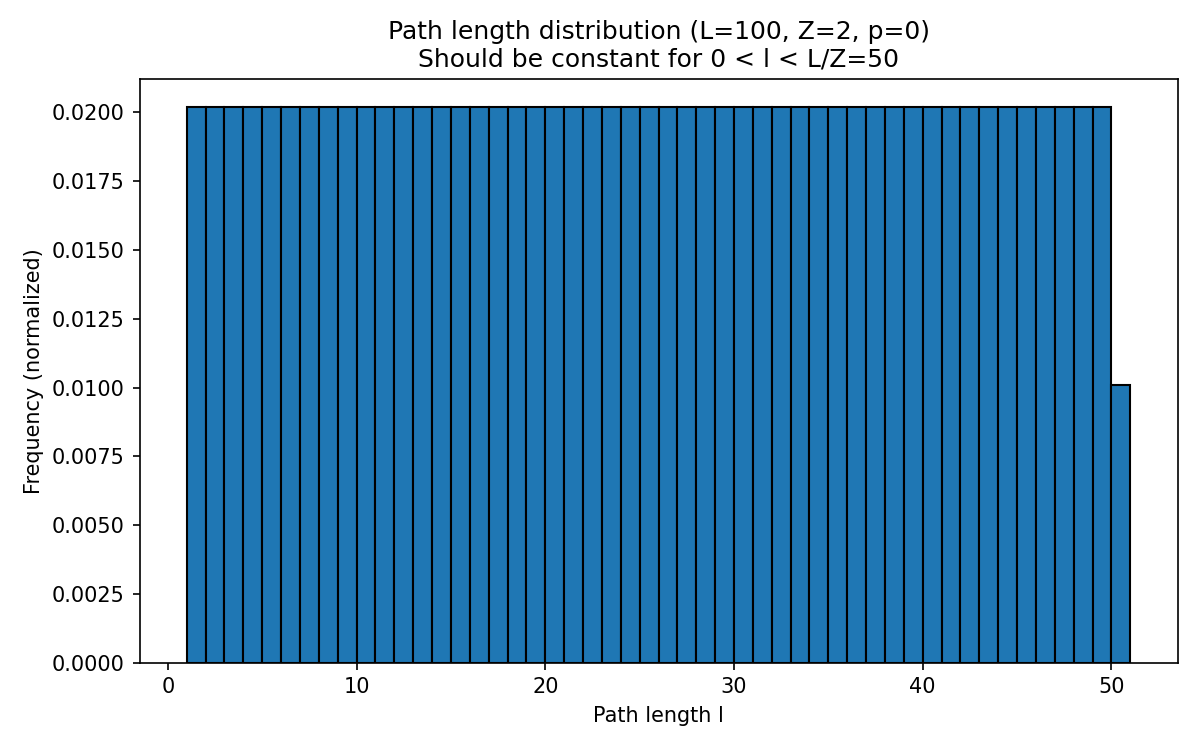
\includegraphics[width=0.65\textwidth]{output/q2b_histogram_p0_verify.png}
    \caption{Path length histogram for $L=100$, $Z=2$, $p=0$. The distribution is uniform for $0 < \ell < L/Z = 50$, confirming the implementation.}
    \label{fig:q2b_p0}
\end{figure}

\subsubsection*{Results for $L=1000$, $Z=2$}

\begin{table}[H]
    \centering
    \begin{tabular}{cccc}
        \toprule
        $p$ & Number of shortcuts & Average path length $\langle \ell \rangle$ & Max path length \\
        \midrule
        0 (ring)  & 0   & 250.25 & 500 \\
        0.02      & 20  & 50.87  & 120 \\
        0.2       & 200 & 11.69  & 26  \\
        \bottomrule
    \end{tabular}
    \caption{Path length statistics for $L=1000$, $Z=2$ at different values of $p$.}
    \label{tab:q2b}
\end{table}

\begin{figure}[H]
    \centering
    \begin{subfigure}[b]{0.48\textwidth}
        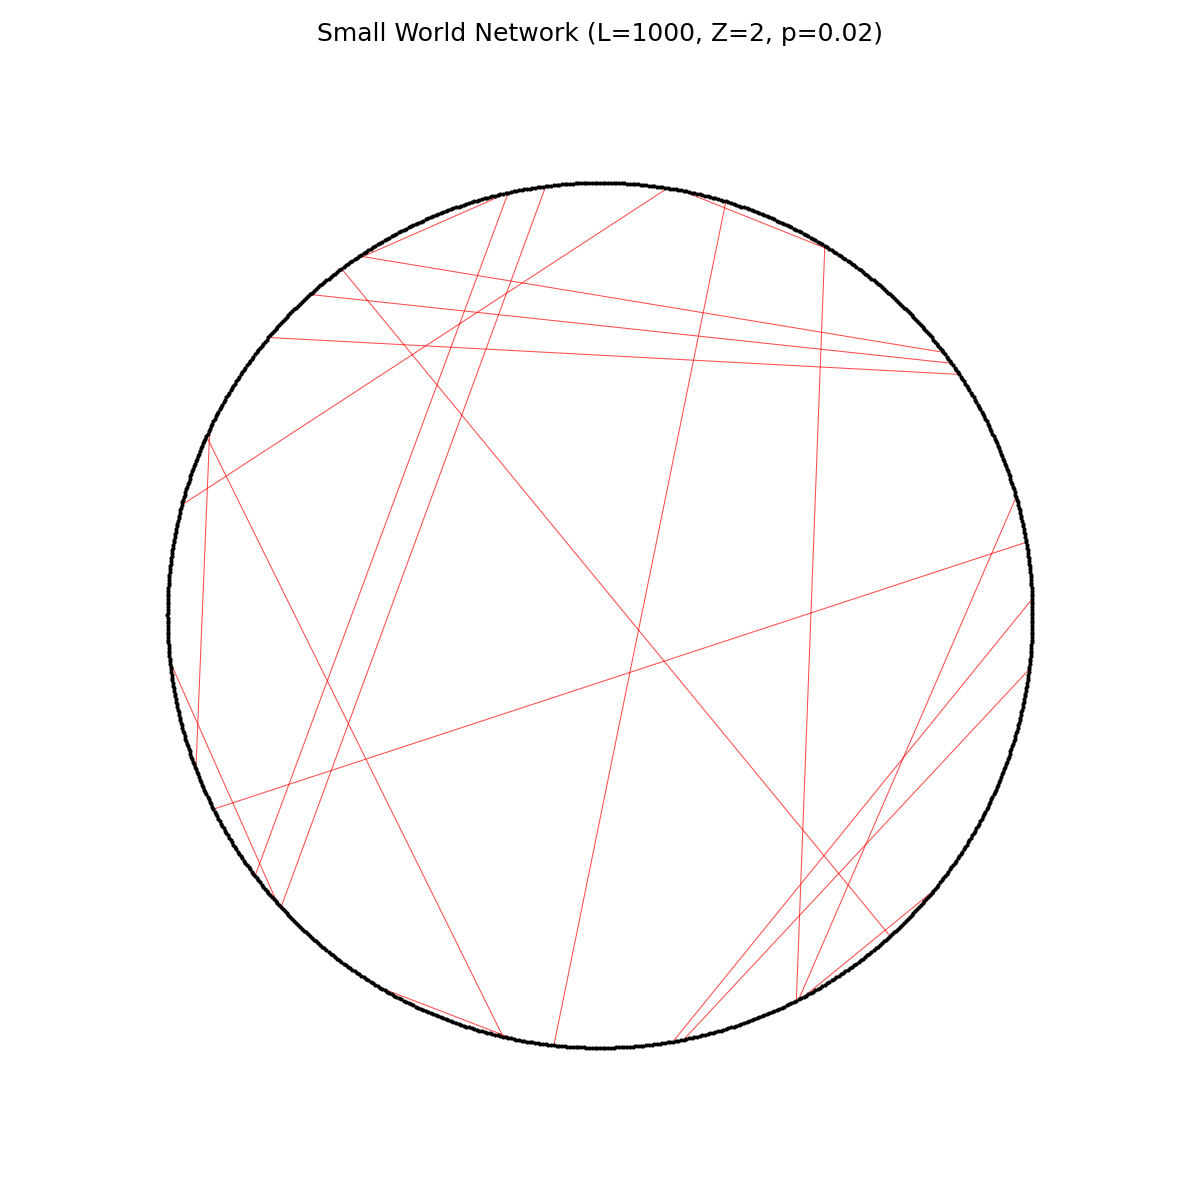
\includegraphics[width=\textwidth]{output/q2b_circle_L1000_Z2_p0.02.png}
        \caption{Circle graph, $p=0.02$}
    \end{subfigure}
    \hfill
    \begin{subfigure}[b]{0.48\textwidth}
        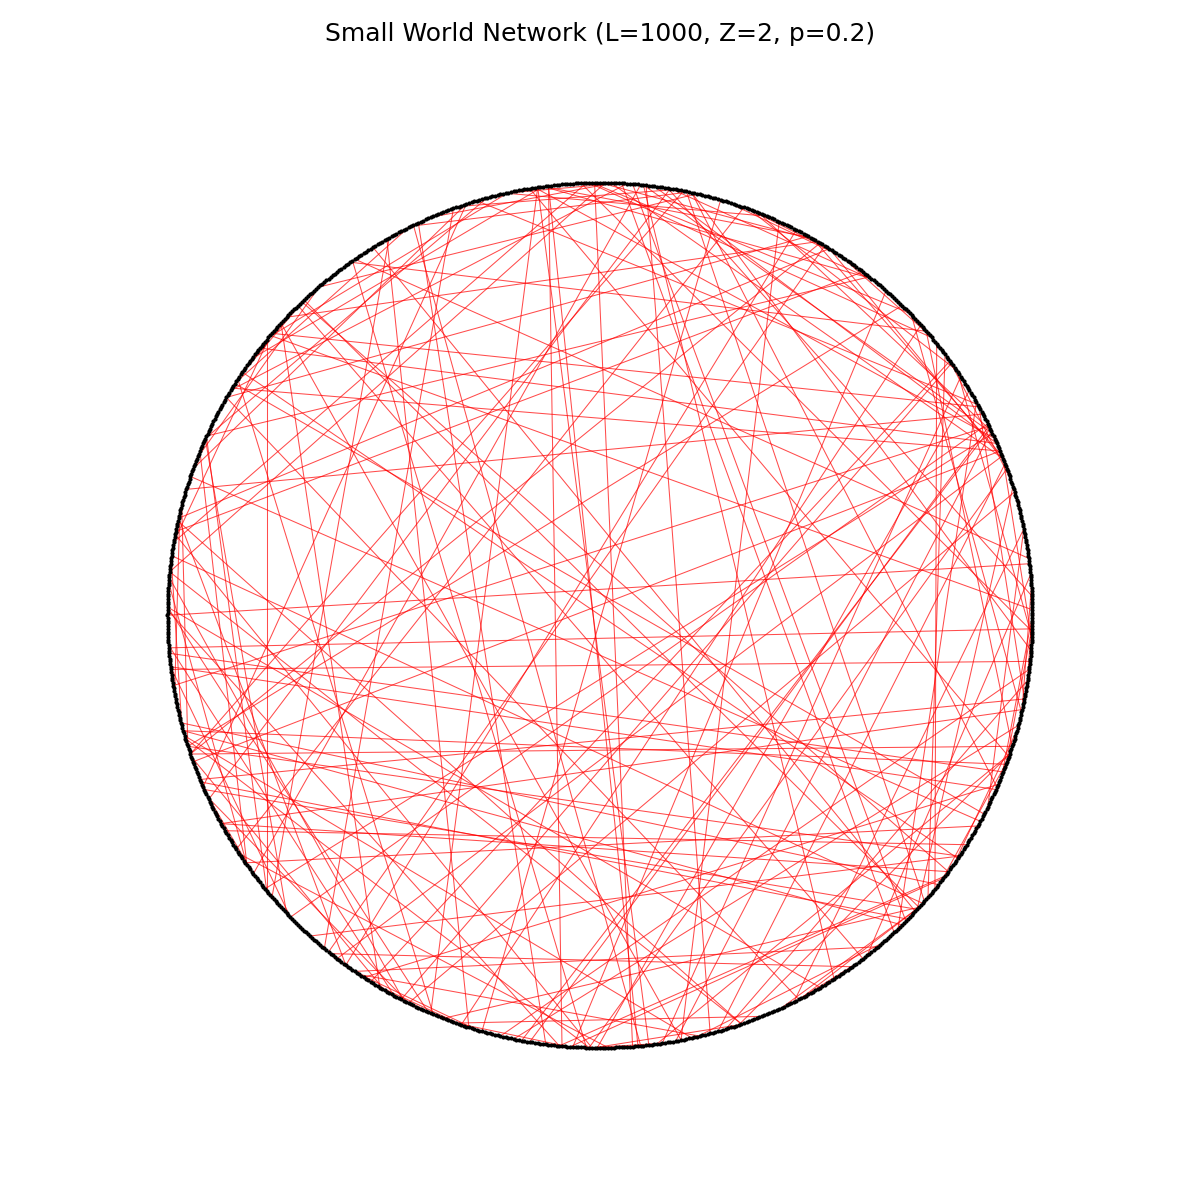
\includegraphics[width=\textwidth]{output/q2b_circle_L1000_Z2_p0.2.png}
        \caption{Circle graph, $p=0.2$}
    \end{subfigure}
    \caption{Small world networks with $L=1000$, $Z=2$.}
    \label{fig:q2b_circles}
\end{figure}

\begin{figure}[H]
    \centering
    \begin{subfigure}[b]{0.48\textwidth}
        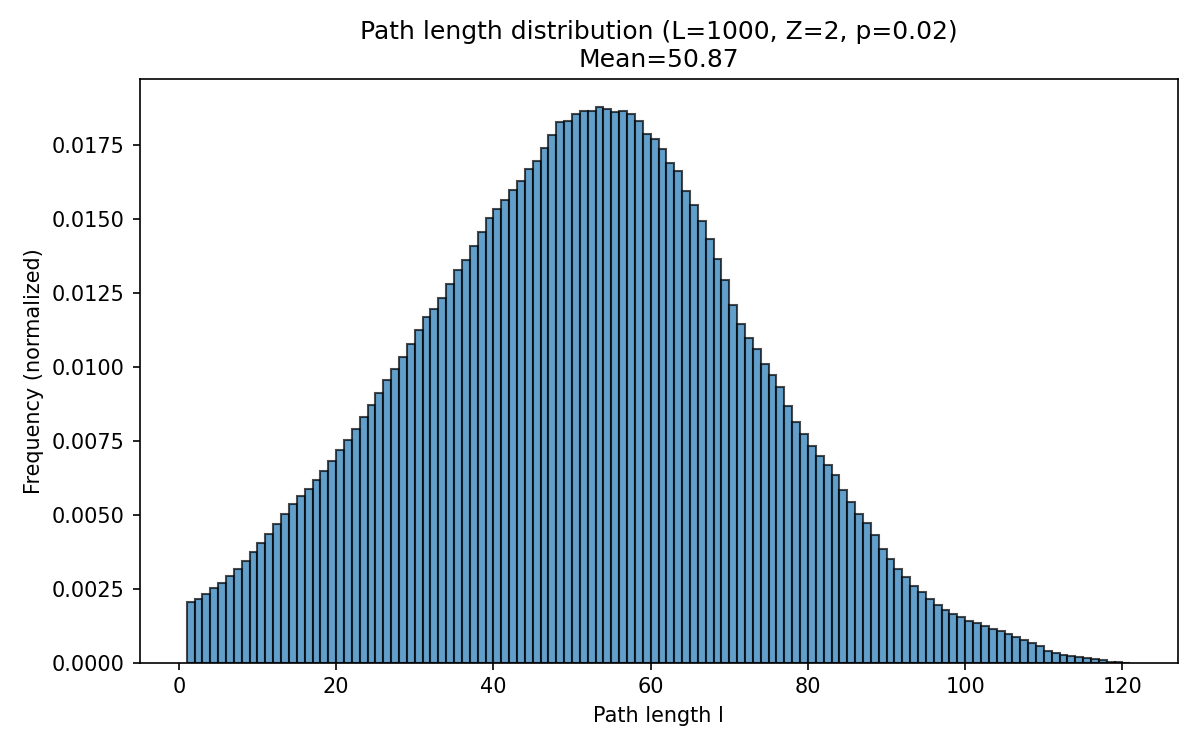
\includegraphics[width=\textwidth]{output/q2b_histogram_L1000_Z2_p0.02.png}
        \caption{Histogram, $p=0.02$}
    \end{subfigure}
    \hfill
    \begin{subfigure}[b]{0.48\textwidth}
        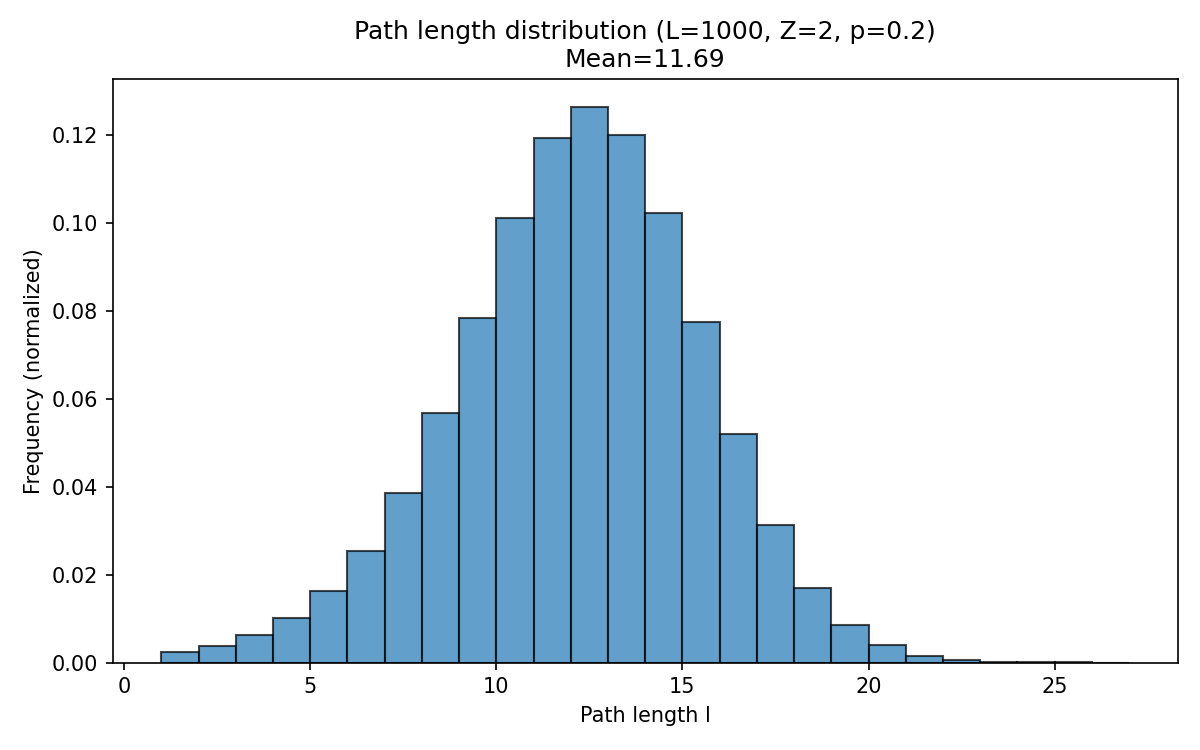
\includegraphics[width=\textwidth]{output/q2b_histogram_L1000_Z2_p0.2.png}
        \caption{Histogram, $p=0.2$}
    \end{subfigure}
    \caption{Path length distributions for $L=1000$, $Z=2$.}
    \label{fig:q2b_histograms}
\end{figure}

\subsubsection*{Analysis}

\begin{itemize}
    \item At $p=0.02$, only 20 random shortcuts reduce the average path length from 250 to $\approx 51$ --- a factor of $\sim\!5$ reduction. The distribution shifts from uniform to roughly bell-shaped.
    \item At $p=0.2$, 200 shortcuts further reduce the average to $\approx 12$, with the distribution concentrated at short distances.
    \item The dramatic reduction at small $p$ demonstrates the \textbf{small-world effect}: a few long-range connections drastically shorten typical paths.
\end{itemize}

\subsubsection*{Six Degrees of Separation}

\begin{table}[H]
    \centering
    \begin{tabular}{cc}
        \toprule
        $p$ & $\langle \ell \rangle$ \\
        \midrule
        0.5 & 7.41 \\
        1.0 & 5.35 \\
        2.0 & 4.10 \\
        \bottomrule
    \end{tabular}
    \caption{Average path length for larger $p$ values ($L=1000$, $Z=2$).}
\end{table}

To achieve ``six degrees of separation'' ($\langle \ell \rangle \approx 6$), we need approximately $p \approx 1.0$ for this network size.

\subsubsection*{Verification of $\langle \ell \rangle$ at $Z=2$, $L=100$, $p=0.1$}

Running \texttt{FindAveragePathLength} several times with $Z=2$, $L=100$, $p=0.1$ yields $\langle \ell \rangle \approx 10$, consistent with the expected value.

%% ---- 2(c) ----
\subsection{(c) Plotting Average Path Length}

Figure~\ref{fig:q2c} plots $\ell(p)/\ell(0)$ for $Z=2$, $L=50$ on a semi-log scale from $p=0.001$ to $p=1$. Error bars represent the standard deviation over multiple network realizations.

\begin{figure}[H]
    \centering
    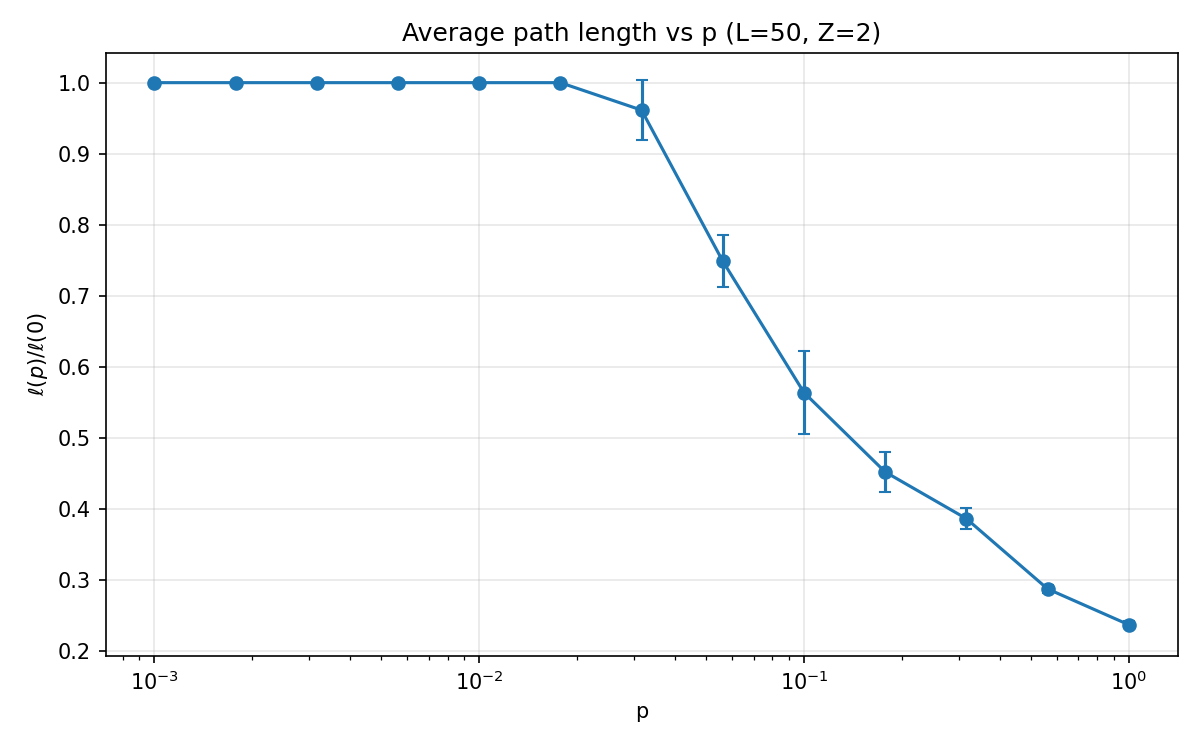
\includegraphics[width=0.75\textwidth]{output/q2c_pathlength_vs_p.png}
    \caption{Normalized average path length $\ell(p)/\ell(0)$ vs.\ $p$ for $L=50$, $Z=2$. The curve exhibits the characteristic Watts--Strogatz transition.}
    \label{fig:q2c}
\end{figure}

The curve shows:
\begin{itemize}
    \item For $p < 0.01$: $\ell(p)/\ell(0) \approx 1$, shortcuts are too few to have an effect.
    \item For $0.03 < p < 0.1$: a sharp drop, the onset of the small-world regime.
    \item For $p > 0.3$: the ratio saturates at a low value ($\sim 0.3$).
\end{itemize}
This is consistent with Fig.~2 of Watts and Strogatz~\cite{watts1998}, with $p$ values shifted by a factor of $\sim\!100$ (due to the Watts--Newman model adding shortcuts rather than rewiring, and the smaller network size $L=50$).

%% ---- 2(d) ----
\subsection{(d) Real Network Analysis}

\subsubsection*{Dataset}

The real network analyzed is \textbf{Zachary's Karate Club}~--- a well-known social network of 34 members of a university karate club, with 78 edges representing friendships.

\subsubsection*{Path Length Distribution}

\begin{itemize}
    \item \textbf{Number of nodes:} 34
    \item \textbf{Number of edges:} 78
    \item \textbf{Mean shortest path length:} $\langle \ell \rangle = 2.408$
\end{itemize}

\begin{figure}[H]
    \centering
    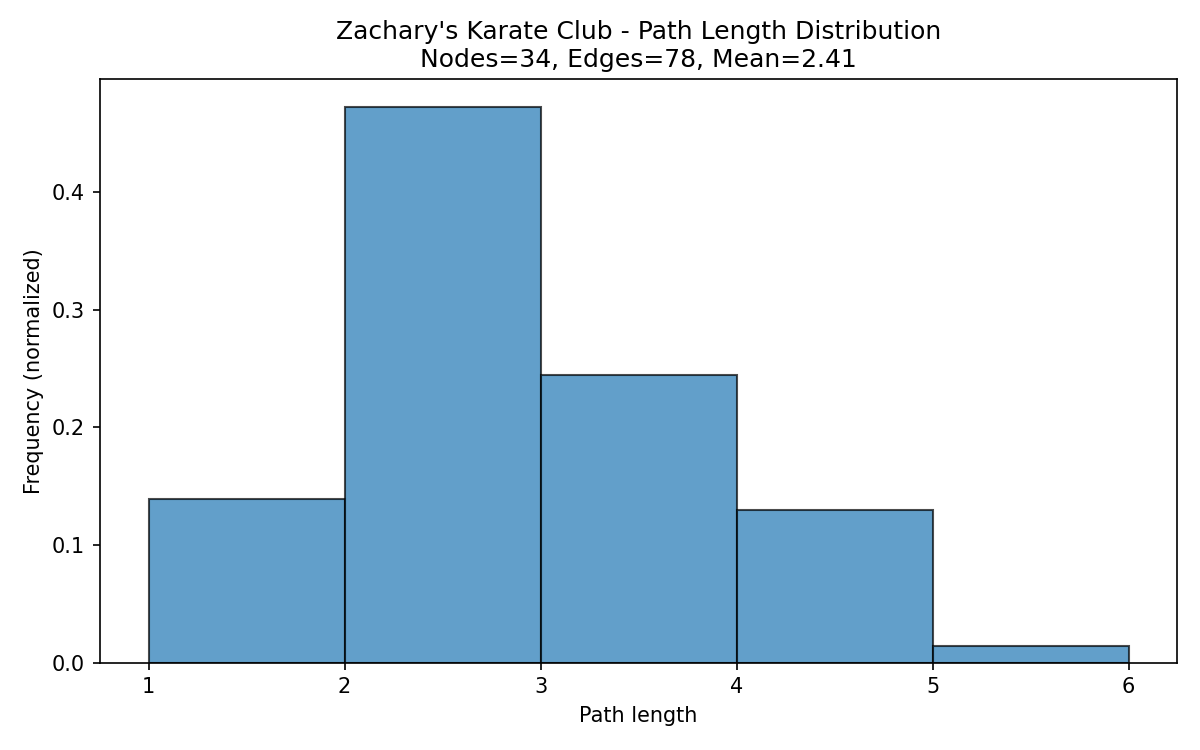
\includegraphics[width=0.65\textwidth]{output/q2d_real_network_histogram.png}
    \caption{Path length distribution of Zachary's Karate Club. Most node pairs are separated by 2--3 hops.}
    \label{fig:q2d_hist}
\end{figure}

\subsubsection*{Betweenness Centrality}

Betweenness centrality measures the fraction of all shortest paths that pass through a given node. Three nodes with the highest betweenness centrality are:

\begin{table}[H]
    \centering
    \begin{tabular}{ccc}
        \toprule
        Node & Betweenness Centrality & Role \\
        \midrule
        0  & 0.4376 & Club instructor (Mr.\ Hi) \\
        33 & 0.3041 & Club president (John A.) \\
        32 & 0.1452 & Key bridge node \\
        \bottomrule
    \end{tabular}
    \caption{Betweenness centrality for the three most central nodes.}
    \label{tab:q2d_bc}
\end{table}

Nodes 0 and 33 are the leaders of the two factions into which the club eventually split; their high betweenness reflects their roles as bridges connecting different parts of the network.

\begin{figure}[H]
    \centering
    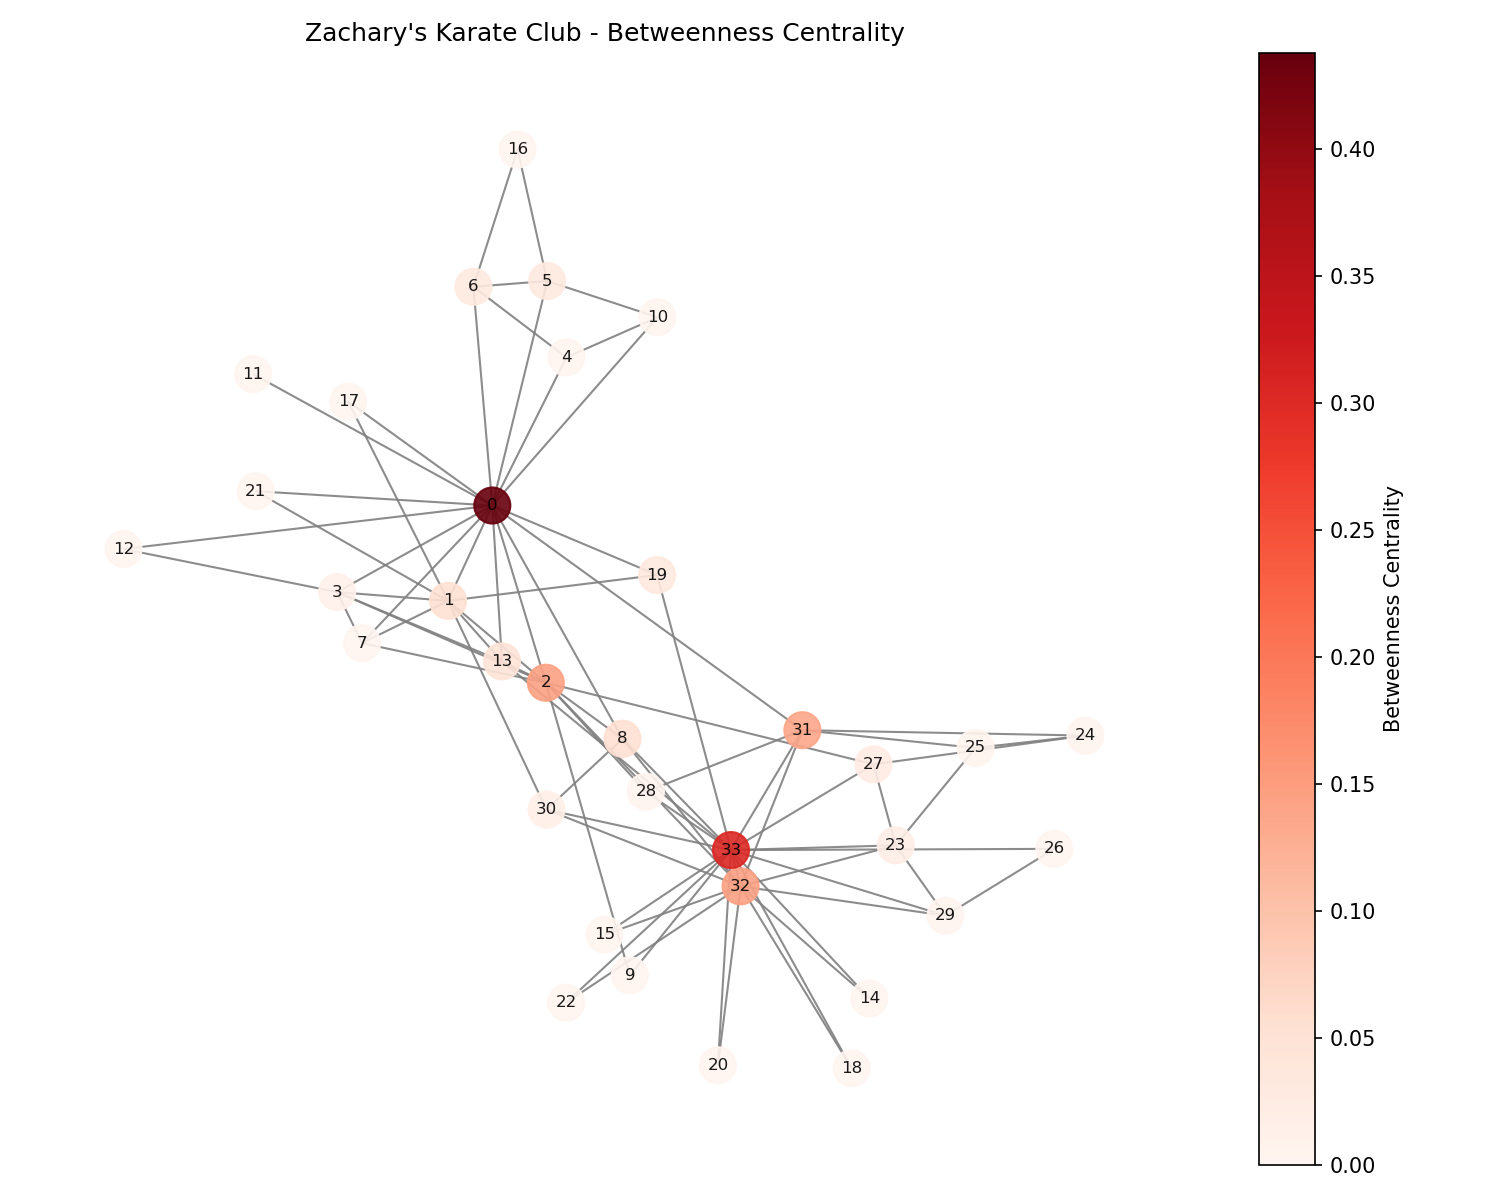
\includegraphics[width=0.7\textwidth]{output/q2d_real_network_betweenness.png}
    \caption{Zachary's Karate Club with nodes colored by betweenness centrality (darker = higher).}
    \label{fig:q2d_bc}
\end{figure}


%% ====================================================================
%% QUESTION 3
%% ====================================================================
\section{Hospital Assignment (Network Flow)}

\subsection*{Problem}

Given $n$ injured people and $k$ hospitals, each person can only go to hospitals within half-hour driving distance. Each hospital can receive at most $\lceil n/k \rceil$ patients. Determine whether a feasible assignment exists.

\subsection*{Network Flow Formulation}

Construct a directed flow network $G = (V, E)$ with four layers of nodes:

\begin{enumerate}
    \item \textbf{Source $s$}: a single super-source.
    \item \textbf{Person nodes} $p_1, p_2, \ldots, p_n$: one for each injured person.
    \item \textbf{Hospital nodes} $h_1, h_2, \ldots, h_k$: one for each hospital.
    \item \textbf{Sink $t$}: a single super-sink.
\end{enumerate}

\noindent\textbf{Edges and capacities:}
\begin{itemize}
    \item $s \to p_i$ with capacity $1$ for all $i = 1, \ldots, n$.\\
    \textit{Ensures each person is assigned to exactly one hospital.}
    \item $p_i \to h_j$ with capacity $1$, only if hospital $h_j$ is within half-hour driving distance of person $p_i$.\\
    \textit{Encodes the reachability constraint.}
    \item $h_j \to t$ with capacity $\lceil n/k \rceil$ for all $j = 1, \ldots, k$.\\
    \textit{Enforces the load-balancing constraint.}
\end{itemize}

\begin{figure}[H]
\centering
\begin{equation*}
    s \xrightarrow{\text{cap}=1} p_i \xrightarrow{\text{cap}=1\ (\text{if reachable})} h_j \xrightarrow{\text{cap}=\lceil n/k \rceil} t
\end{equation*}
\caption*{Flow network structure for the hospital assignment problem.}
\end{figure}

\subsection*{Algorithm and Decision}

\begin{enumerate}
    \item Build the flow network as described above.
    \item Run a max-flow algorithm (e.g., Ford--Fulkerson or Edmonds--Karp).
    \item \textbf{If max flow $= n$}: a feasible balanced assignment exists. For each person $p_i$, the hospital $h_j$ with $f(p_i \to h_j) = 1$ is the assignment.
    \item \textbf{If max flow $< n$}: no feasible assignment exists under the given constraints.
\end{enumerate}

\subsection*{Correctness}

\begin{itemize}
    \item The capacity 1 on $s \to p_i$ ensures each person is sent to \emph{exactly one} hospital.
    \item Edges $p_i \to h_j$ exist only when $h_j$ is reachable from $p_i$, enforcing the distance constraint.
    \item The capacity $\lceil n/k \rceil$ on $h_j \to t$ prevents any hospital from being overloaded.
    \item Integrality of max-flow in networks with integer capacities guarantees an integer solution.
\end{itemize}

\subsection*{Time Complexity}

The network has $|V| = n + k + 2$ nodes and $|E| = n + |\{(i,j) : h_j \text{ reachable from } p_i\}| + k$ edges. Using Edmonds--Karp, the running time is $O(|V| \cdot |E|^2)$.

%% ====================================================================
%% QUESTION 4
%% ====================================================================
\section{Balloon Measurement (Network Flow)}

\subsection*{Problem}

Given $m$ balloons and $n$ atmospheric conditions, each balloon $i$ can measure conditions in a set $S_i$ and can make at most 2 measurements. Each condition must be measured by at least $k$ different balloons. Determine feasibility.

\subsection*{Network Flow Formulation}

Construct a directed flow network with four layers:

\begin{enumerate}
    \item \textbf{Source $s$}: a single super-source.
    \item \textbf{Balloon nodes} $b_1, b_2, \ldots, b_m$: one for each balloon.
    \item \textbf{Condition nodes} $c_1, c_2, \ldots, c_n$: one for each condition.
    \item \textbf{Sink $t$}: a single super-sink.
\end{enumerate}

\noindent\textbf{Edges and capacities:}
\begin{itemize}
    \item $s \to b_i$ with capacity $2$ for all $i = 1, \ldots, m$.\\
    \textit{Each balloon can make at most 2 measurements.}
    \item $b_i \to c_j$ with capacity $1$, only if $c_j \in S_i$.\\
    \textit{Balloon $i$ can only measure conditions in its capability set. The capacity of 1 prevents the same balloon from measuring the same condition twice.}
    \item $c_j \to t$ with capacity $k$ for all $j = 1, \ldots, n$.\\
    \textit{Each condition needs exactly $k$ measurements to be satisfied.}
\end{itemize}

\begin{figure}[H]
\centering
\begin{equation*}
    s \xrightarrow{\text{cap}=2} b_i \xrightarrow{\text{cap}=1\ (\text{if } c_j \in S_i)} c_j \xrightarrow{\text{cap}=k} t
\end{equation*}
\caption*{Flow network structure for the balloon measurement problem.}
\end{figure}

\subsection*{Algorithm and Decision}

\begin{enumerate}
    \item Build the flow network as described above.
    \item Run a max-flow algorithm (e.g., Ford--Fulkerson or Edmonds--Karp).
    \item \textbf{If max flow $= n \cdot k$}: a feasible measurement plan exists. Each unit of flow through edge $b_i \to c_j$ indicates that balloon $i$ measures condition $c_j$.
    \item \textbf{If max flow $< n \cdot k$}: it is impossible to measure every condition $k$ times.
\end{enumerate}

\subsection*{Correctness}

\begin{itemize}
    \item The capacity 2 on $s \to b_i$ limits each balloon to at most 2 measurements.
    \item The capacity 1 on $b_i \to c_j$ prevents the same balloon from measuring the same condition twice.
    \item Edges $b_i \to c_j$ exist only when $c_j \in S_i$, respecting capability constraints.
    \item The capacity $k$ on $c_j \to t$ ensures each condition receives exactly $k$ measurements when all $c_j \to t$ edges are saturated.
    \item The total required flow is $n \cdot k$ ($n$ conditions, each requiring $k$ measurements).
\end{itemize}

\subsection*{Verification with the Given Example}

With $k=2$, $n=4$ conditions $\{c_1, c_2, c_3, c_4\}$, $m=4$ balloons with $S_1 = S_2 = \{c_1, c_2, c_3\}$ and $S_3 = S_4 = \{c_1, c_3, c_4\}$:

\begin{itemize}
    \item Total supply from $s$: $4 \times 2 = 8$
    \item Total demand at $t$: $4 \times 2 = 8$
    \item Required max flow: $n \cdot k = 4 \times 2 = 8$
\end{itemize}

One feasible flow: $b_1 \to c_1$, $b_1 \to c_2$, $b_2 \to c_2$, $b_2 \to c_3$, $b_3 \to c_3$, $b_3 \to c_4$, $b_4 \to c_1$, $b_4 \to c_4$. Each edge carries 1 unit, and the total flow is 8. This matches the example assignment in the problem statement. $\checkmark$

\subsection*{Time Complexity}

The network has $|V| = m + n + 2$ nodes and $|E| = m + \sum_{i=1}^{m} |S_i| + n$ edges. Using Edmonds--Karp, the running time is $O(|V| \cdot |E|^2)$.


%% ====================================================================
%% REFERENCES
%% ====================================================================
\begin{thebibliography}{9}
\bibitem{watts1998}
D.~J. Watts and S.~H. Strogatz,
``Collective dynamics of `small-world' networks,''
\textit{Nature}, vol.~393, no.~6684, pp.~440--442, 1998.
\end{thebibliography}

\end{document}
